\section{Equazione del calore e la sua approssimazione numerica}
L'equazione del calore, come facilmente intuibile, è stata formulata per determinare l'evoluzione di un sistema isolato che presenta al suo interno una data distribuzione di calore. La sua rappresentazione differenziale è la seguente:\\
$$
\begin{cases}
\frac{\partial u}{\partial t}(t,x)-\Delta u(t,x) = 0 \ x \in \mathbb R^2, t\ge 0 \ .\\ 
u(0,x) = u_0(x)\ . \\
\end{cases}
$$
Euristicamente, non è difficile pensare che si possano codificare (pensando ad un'immagine in bianco e nero) i pixel più luminosi come punti \textit{"più caldi"}, mentre quelli più scuri come punti \textit{"più freddi"} ed applicare così l'equazione del calore all'immagine.\\
Mediante uno script MATLAB si può dunque osservare come quest'ultima operi nella pratica, sfruttando una approssimazione alle \textbf{differenze finite } utile per il calcolo delle derivate.\\
\vspace{-0.5em}
\subsection{Metodo delle differenze finite}
\raggedright
Il metodo delle differenze finite, come anticipato, viene impiegato nel calcolo approssimato delle derivate. 
\vspace{-0.5em}
\begin{definizione}

Data una generica funzione u, consideriamone lo sviluppo di Taylor\\
\vspace{0.25em}
\centering
$u(x_i+\Delta(x))=u(x_i)+u'(x_i)\Delta(x)+\frac{1}{2}u''(x_i)\Delta(x)^2+o(h^2)$ \\
\vspace{0.25em}
\raggedright
La scelta adottata per la suddetta approssimazione risulterà dunque essere:\\
\vspace{0.25em}
\centering 
$\frac{du}{dx}\approx\frac{u(x+\Delta(x))-u(x)}{\Delta(x)} \approx \frac{u_{i+1} - u_i}{\Delta(x)} $.
\footnote{\cite{FD}}\\
\vspace{0.25em}
\raggedright
Tale approssimazione è detta \textbf{differenza finita in avanti}. Analogamente si trova, come approssimazione altrettanto valida la \textbf{differenza finita all'indietro}:\\
\vspace{0.25em}
\centering 
$\frac{du}{dx}\approx\frac{u(x)-u(x-\Delta(x))}{\Delta(x)} \approx \frac{u_i - u_{i-1}}{\Delta(x)} $.\\
\vspace{0.25em}
\raggedright
\end{definizione}
\begin{definizione}
Consideriamo adesso gli sviluppi di Taylor che hanno portato alle formule di approssimazione alle differenze finite appena viste e sottraiamo membro a membro.\\
\vspace{0.25em}
\centering
$u(x_i+\Delta(x))=u(x_i)+u'(x_i)\Delta(x)+\frac{1}{2}u''(x_i)\Delta(x)^2+\frac{1}{6}u'''(x_i)\Delta(x)^3+o(\Delta(x)^3)$ \\
\vspace{0.25em}
$u(x_i-\Delta(x))=u(x_i)-u'(x_i)\Delta(x)+\frac{1}{2}u''(x_i)\Delta(x)^2-\frac{1}{6}u'''(x_i)\Delta(x)^3+o(\Delta(x)^3)$ \\
$\Downarrow$\\
$u(x_i+\Delta(x))-u(x_i-\Delta(x))=+2u'(x_i)\Delta(x)+2\frac{1}{6}u'''(x_i)\Delta(x)^3+o(\Delta(x)^3)$ \\
\vspace{0.25em}
\raggedright
Questi conti inducono l'approssimazione:\\
\vspace{0.25em}
\centering 
$\frac{du}{dx}\approx\frac{u(x+\Delta(x))-u(x-\Delta(x))}{2\Delta(x)} \approx \frac{u_{i+1} - u_{i-1}}{2\Delta(x)}$\\
\vspace{0.25em}
\raggedright
Tale approssimazione è detta \textbf{differenza finita centrata}.
\end{definizione}

\vspace{1em}
Dal momento che la derivata seconda coincide con la derivata della derivata prima, è intuitivo dare la seguente definizione per la sua approssimazione numerica:
\begin{definizione}
\noindent
Consideriamo la funzione $u$ e l'approssimazione della sua derivata alle differenze finite $\frac{du}{dx}=\frac{u_{i+1} - u_i}{\Delta(x)}$, applicando ad esso il metodo delle differenze finite troviamo: 
\begin{align*}
\frac{d^2u}{dx^2} \approx &
\frac{
(\frac{u_{i+1} - u_i}{\Delta(x)})_{i+1} 
- 
(\frac{u_{i+1} - u_i}{\Delta(x)})_i
}{\Delta(x)}
=
\frac{
\frac{(u_{i+1} - u_i)_{i+1}}{\Delta(x)} 
-   
\frac{(u_{i+1} - u_i)_i}{\Delta(x)}
}{\Delta(x)}
\\
\vline&
\\
= &
\frac{
\frac{(u_{i+2} - u_{i+1})}{\Delta(x)} 
- 
\frac{(u_{i+1} - u_i)}{\Delta(x)}
}{\Delta(x)}
=
\frac{
\frac{(u_{i+2} - u_{i+1}) 
- 
(u_{i+1} - u_i)}{\Delta(x)}
}{\Delta(x)}
\\
\vline
\\
= &
\frac{
(u_{i+2} - u_{i+1}) 
- 
(u_{i+1} - u_i)}
{\Delta(x)^2}
=
\frac{
 u_{i+2} - u_{i+1} 
-u_{i+1} + {u_i}}
{\Delta(x)^2}
.\\
\end{align*}
\raggedright
\end{definizione}
\begin{osservazione}
Per ottenere una stima accurata è bene utilizzare un valore di $\Delta(x)$ quanto più basso possibile. La migliore è guardare la differenza tra un pixel e quello adiacente ossia $\Delta(x)=1$, ma allora 

$$\frac{d^2u}{dx^2} \approx
\frac{
 u_{i+2} - u_{i+1} 
-u_{i+1} + u_i}
{\Delta(x)^2} = u_{i+2} -2 u_{i+1} + u_i.$$

\`E chiaro che scorrendo tutti gli indici questo è equivalente a $u_{i+1} -2 u_i + u_{i-1}.$
\end{osservazione}

In sintesi si può utilizzare per il calcolo delle derivate seconde che compongono il laplaciano l'approssimazione\\
$$\frac{d^2u}{dx^2} \approx u_{i+1} -2 u_i + u_{i-1}$$
\newpage
\subsubsection{Errore di troncamento}

Vale la pena di fare qualche considerazione sull'errore di troncamento che si commette adottando queste approssimazioni.\\

\begin{definizione}
Definiamo \textbf{errore} o più precisamente \textbf{errore assoluto} $\epsilon$ di un'approssimazione $u'$ di un valore d'interesse $u$ la differenza $\epsilon=u-u'$, cioè tra il valore esatto e quello approssimato.
\end{definizione}
Per quanto riguarda le derivate prime basta guardare agli sviluppi di Taylor che ci hanno portato alle loro approssimazioni per osservare che\\
\begin{osservazione}
Applicando la definizione di errore assoluto alle diverse approssimazioni finora definite per le derivate di primo grado troviamo:
\begin{itemize}
    \item Differenza finita in avanti\\
    \centering
    $u(x_i+\Delta(x))=u(x_i)+u'(x_i)\Delta(x)+\frac{1}{2}u''(x_i)\Delta(x)^2+o(\Delta(x)^2)$ \\ $\Downarrow$\\
    $\epsilon=\frac{u(x_i+\Delta(x))-u(x_i)}{\Delta(x)} -u'(x_i)\approx \frac{1}{2}u''(x_i)\Delta(x)$\\
    \raggedright
    \item Differenza finita all'indietro\\
    \centering
    $u(x_i-\Delta(x))=u(x_i)-u'(x_i)\Delta(x)+\frac{1}{2}u''(x_i)\Delta(x)^2+o(\Delta(x)^2)$ \\ $\Downarrow$\\
    $\epsilon=\frac{u(x_i)-u(x_i-\Delta(x))}{\Delta(x)} -u'(x_i)\approx \frac{1}{2}u''(x_i)\Delta(x)$\\
    \raggedright
    \item Differenza finita centrata\\
    \centering
    $u(x_i+\Delta(x))-u(x_i-\Delta(x))=+2u'(x_i)\Delta(x)+2\frac{1}{6}u'''(x_i)\Delta(x)^3+o(\Delta(x)^3)$ \\ $\Downarrow$\\
    $\epsilon=\frac{u(x_i+\Delta(x))-u(x_i-\Delta(x))}{2\Delta(x)} -u'(x_i)\approx +\frac{1}{6}u'''(x_i)\Delta(x)^2$\\
    \raggedright
\end{itemize}
Ad un'attenta analisi possiamo vedere che tra i metodi di approssimazione in avanti, in indietro o centrale, il calcolo dell'errore portato dai primi due sono uguali tra di loro, quello centrale invece è diverso, esso dipende da un $\Delta(x)^2$ e non da un $\Delta(x)$, questo vuol dire che per $\Delta(x)<1$ funziona meglio, per $\Delta(x)>1$ funziona peggio. Nel caso in analisi $\Delta(x)=1$ quindi la scelta è indifferente.
\end{osservazione}
Per quanto riguarda la derivata seconda invece
\begin{osservazione}
Applicando la definizione di errore per la formula alle derivate finite per l'approssimazione della la derivata seconda:
$$
\epsilon= \frac{u_{i+1}-2u_{i}+u_{i-1}}{\Delta(x)^2} - u''_i
$$
Da questa rappresentazione non riusciamo purtroppo a dedurre nulla, proviamo quindi con un altro metodo. Consideriamo lo sviluppo di Taylor troncato al quarto ordine
$$
u_{i+1}=u_i+u'_i\Delta(x)+\frac{1}{2}u''_i\Delta(x)^2+\frac{1}{6}u'''_i\Delta(x)^3 + \frac{1}{24}u''''_i\Delta(x)^4 +o(\Delta(x)^4)
$$
$$
-\frac{1}{2}u''_i\Delta(x)^2=-u_{i+1} + u_i + u'_{i}\Delta(x) + \frac{1}{6}u'''_i\Delta(x)^3 + \frac{1}{24}u''''_i\Delta(x)^4 +o(\Delta(x)^4)
$$
$$
-\frac{1}{2}u''_i\Delta(x)^2 = -u_{i+1} + u_i + (\frac{u_{i+1}-u_{i-1}}{2\Delta(x)} -\frac{1}{6}u'''_i\Delta(x)^2)\Delta(x) + \frac{1}{6}u'''_i\Delta(x)^3 + \frac{1}{24}u''''_i\Delta(x)^4 +o(\Delta(x)^4)
$$
$$
-\frac{1}{2}u''_i\Delta(x)^2 = -u_{i+1} + u_i + \frac{1}{2}u_{i+1} - \frac{1}{2}u_{i-1} -\frac{1}{6}u''_i\Delta(x)^3 + \frac{1}{6}u'''_i\Delta(x)^3 + \frac{1}{24}u''''_i\Delta(x)^4 +o(\Delta(x)^4)
$$
$$
-\frac{1}{2}u''_i\Delta(x)^2 = -\frac{1}{2}u_{i+1} + u_i - \frac{1}{2}u_{i-1} + \frac{1}{24}u''''_i\Delta(x)^4 +o(\Delta(x)^4)
$$
$$
\epsilon=-u''_i + \frac{u_{i+1} - 2u_i + u_{i-1}}{\Delta(x)^2} \approx \frac{1}{12}u''''_i\Delta(x)^2
$$
Risulta quindi evidente che l'errore dipende da $\Delta(x)^2$. 
\end{osservazione}

%$$
%\frac{d^2u}{dx^2}\vline_{x_i}-\frac{u_{i+1}-u_i}{\Delta(x)}\approx \frac{\Delta(x)^2}{2} \frac{d^2u}{dx^2}\vline_\xi.
%$$

%Ma procediamo con ordine.\\

Per brevità di notazione poniamo d'ora in poi $\Delta(x)=h$.\\
\begin{proposizione}
Dato un problema differenziale $-u'' + \sigma u=f$ con condizioni al contorno di Dirichlet $g_0$ e $g_1$, allora se $\sigma\geq0$ la risoluzione del problema tramite metodo delle differenze finite è convergente.
\end{proposizione}

\begin{proof}
Senza ledere di generalità possiamo assumere che $u,f,\sigma$ definite su $I=(0,1)$, il problema assume quindi la forma

$$
\begin{cases}
-u'' + \sigma u=f\\
u(0)=g_0\\
u(1)=g_1
\end{cases}
$$

Per quanto visto nell'osservazione 2.1.3 possiamo scrivere
$$
u''(x_j) =\frac{u(x_{j+1}) - 2u(x_j) + u(x_{j-1})}{h^2} -\frac{1}{12} u^{(4)}(\xi_j)h^2
$$
dove $\xi_j$ e un punto opportuno in $(x_{j-1} , x_{j+1})$. Allora per $j = 1,...,N-1$, si può scrivere che

$$
\frac{-u(x_{j+1}) + 2u(x_j) -u(x_{j-1})}{h^2}
 + \frac{1}{12} u^{(4)}(\xi_j)h^2 + \sigma(x_j)u(x_j) = f(x_j) .
$$

Introducendo la notazione $\tau_{j}=\frac{1}{12} u''''(\xi_j)h^2$ (errore di troncamento locale) e ponendo:\\

$$\boldsymbol{u}=[u_x...u_{N-1}]^T$$
$$\boldsymbol{\tau_h}=[\tau_x...\tau_{N-1}]^T$$
$$\boldsymbol{b_h}=[(f(x_1) + \frac{g_0}{h^2},f(x_2),...,f(x_{N-2}),f(x_{N-1}) + \frac{g_1}{h^2}]^T$$

si può allora scrivere in forma matriciale,
$A_h\boldsymbol{u} = \boldsymbol{b_h} + \boldsymbol{\tau_h}$
dove $A_h = \frac{1}{h^2}
 tridiag(-1,2,-1) + diag(\sigma_1, ... ,\sigma_{N-1})$ e $\sigma_j = \sigma(x_j)$.\\
\vspace{1em}
Il metodo alle differenze finite consiste allora nel determinare un’approssimazione $u_h$ di
u andando a risolvere il sistema lineare
$A_h\boldsymbol{u_h} = \boldsymbol{b_h}.$
Osserviamo che $\boldsymbol{u_h}$ risulta ben definito in quanto $A_h$ è una matrice non singolare, il che è verificato in quando la matrice è composta da sole righe linearmente indipendenti.\\

\vspace{1em}

Risultando che $\boldsymbol{\tau_h}$ tende a zero quando h tende a zero, il metodo dicesi consistente. In particolare risulta $\boldsymbol{\tau_h} = O(h^2)$.\\
Tuttavia la consistenza non assicura da sola la convergenza del metodo.\\
Per studiarne la convergenza è necessario considerare il comportamento dell’errore $\boldsymbol{\epsilon_h} = \boldsymbol{u_h} -\boldsymbol{u}$ quando h tende a zero. Dato che risulta $A_h\boldsymbol{\epsilon_h} = \boldsymbol{\tau_h}$, e quindi $\boldsymbol{\epsilon_h} = A_h^{-1} \boldsymbol{\tau_h}$ si può quindi scrivere: $\left\|\boldsymbol{\epsilon_h}\right\|\geq \left\|A_h^{-1}\right\| \left\|\boldsymbol{\tau_h}\right\|$\\
Il passaggio successiovo è far vedere che, lavorando in norma infinito, si è in grado di trovare una costante che, per ogni $h$, maggiora $\left\|A_h^{-1}\right\|_{\infty} $. \\ 
A questo scopo osserviamo che si può dimostrare che sia $A_h$ che la matrice $A_{0h} = \frac{1}{h^2} tridiag(-1,2,-1)$ hanno inversa non negativa, e si ha: 

$$A_{0h}^{-1}-A_{h}^{-1}=A_{0h}^{-1}(A_h-A_{0h})A_h^{-1}\geq0.$$

Per come è definita $A_h$, vale la disuguaglianza $\left\|A_h^{-1}\right\|_{\infty} \leq \left\|A_{0h}^{-1}\right\|_{\infty} $
si può quindi osservare che
$\left\|A_{0h}^{-1}\right\|_{\infty} =max_j(A_{0h}^{-1}{ones(N-1)})_j$ dove ${ones(N-1)}$ indica il vettore di tutti 1.\\
Osservando che la soluzione esatta del problema $-u'' = 1, u(0) = u(1) = 0$, è il polinomio di secondo grado $\phi(x) = \frac{x(1-x)}{2}$, si può concludere che $A_{0h}^{-1}(ones(N-1)_j=\phi(x_j)$ e quindi che $\left\|A_h^{-1}\right\|_{\infty} \leq \left\|A_{0h}^{-1}\right\|_{\infty} \leq max_{0<x<1}|\phi_x|$.\\
Questo risultato di stabilità ci permette di concludere che l’errore $\boldsymbol{\epsilon_h}$ ha lo stesso ordine dell’errore di troncamento $\boldsymbol{\tau_h}$ e di conseguenza che il metodo è convergente del secondo ordine.\\
\end{proof}
\begin{osservazione}
Si noti che l’uniforme limitatezza della norma di $A_h^{-1}$ implica che il metodo numerico sia stabile.\\
\end{osservazione}
Questo è un risultato che ha valenza generale, riportato al caso dell'equazione del calore abbiamo che $\frac{\partial u}{\partial t} - \Delta u = \frac{\partial u}{\partial t} - \frac{\partial^2 u}{\partial x^2} - \frac{\partial^2 u}{\partial y^2} = 0$ per cui $-\frac{\partial^2 u}{\partial x^2}=\frac{\partial u}{\partial t}|_x$ e $-\frac{\partial^2 u}{\partial y^2}=\frac{\partial u}{\partial t}|_y$. Per entrambe le equazioni trovate ci troviamo nel caso $\sigma=0$ e quindi in particolare $\sigma\geq0$, in queste condizioni $\left\|A_h^{-1}\right\|_{\infty} = \left\|A_{0h}^{-1}\right\|_{\infty} $ e quindi in particolare $\left\|A_h^{-1}\right\|_{\infty} \leq \left\|A_{0h}^{-1}\right\|_{\infty} $, la condizione di convergenza è dunque soddisfatta.


\newpage

\subsection{L'equazione del calore}

\raggedright

Il metodo delle differenze finite sarà impiegato in uno script MATLAB per l'implementazione dell'equazione del calore, è bene quindi prenderla in esame.


$$
\begin{cases}
\frac{\partial u}{\partial t}(t,x)-\Delta u(t,x) = 0 \ x \in \mathbb R^2, t\ge 0 \ .\\ 
u(0,x) = u_0(x)\ . \\
\end{cases}
$$

Ricordiamo $\Delta u=\frac{\partial^2u}{\partial x^2}+\frac{\partial^2u}{\partial y^2}$ per cui la sua approssimazione numerica sarà:
$$
u_{i,j}^{n+1}=u_{i,j}^{n}+k_x \Delta t(u_{i+1,j}^{n}-2u_{i,j}^{n}+u_{i-1,j}^{n})+k_y \Delta t(u_{i,j+1}^{n}-2u_{i,j}^{n}+u_{i,j-1}^{n})
$$
Con $k_x$ e $k_y$ coefficienti di controllo (nello script porremo $k_x=k_y=k$).\\
L'equazione del calore, come anticipato, determina l'evoluzione di un sistema isolato che presenta al suo interno una data distribuzione di calore. \`E banale pensare che con il passare del tempo il calore si distribuisca, tendendo per un tempo infinito ad una distribuzione uniforme.

\vspace{1em}

Applicando l'equazione del calore si ottiene quindi un'immagine sempre più \textit{"liscia"}, di fatto una sfocatura, e per un numero di iterazioni idealmente infinito si giungerebbe ad una distribuzione uniforme di colore, ossia una tinta unita.

\vspace{1em}
%\newpage

Il seguente script MATLAB illustra come questo processo opera nella pratica.

\begin{lstlisting}[language=MATLAB]
Im=imread('parrot.jpeg');   %Apro l'immmagine
Im=rgb2gray(Im);            %La trasformo in bianco e nero
Im=imnoise(Im,'gaussian');  %Aggiungo del rumore

%---Definisco le costanti e le condizioni iniziali

[ny, nx, ~]=size(Im)        %Dimensioni dell'immagine
dt=0.25;                    %Passo temporale
u=double(Im);               %Copia dell'immagine originale su cui                                lavorare
T=3			                    %Tempo, ossia T/dt + 1 definisce il numero                           di iterazioni da eseguire
k=0.5;

%---Mostro l'immagine originale
imshow(uint8(Im))
title('immagine originale'); 

%---Metodo eq del calore
u=double(Im);
for t = 0:dt:T
   u_xx = u(:,[2:nx nx],:) - 2*u + u(:,[1 1:nx-1],:);  % derivata                                                           seconda lungo x
   u_yy = u([2:ny ny],:,:) - 2*u + u([1 1:ny-1],:,:);  % derivata                                                           seconda lungo y
   u= u + k*dt*(u_xx+u_yy);
   temp=u;
end

\end{lstlisting}
%\vspace{1em}
\newpage
Provando a cambiare il tempo, ossia il numero di iterazioni, si può osservare come un maggior lasso di tempo produca immagini più sfocate.

\begin{figure} 
\centering
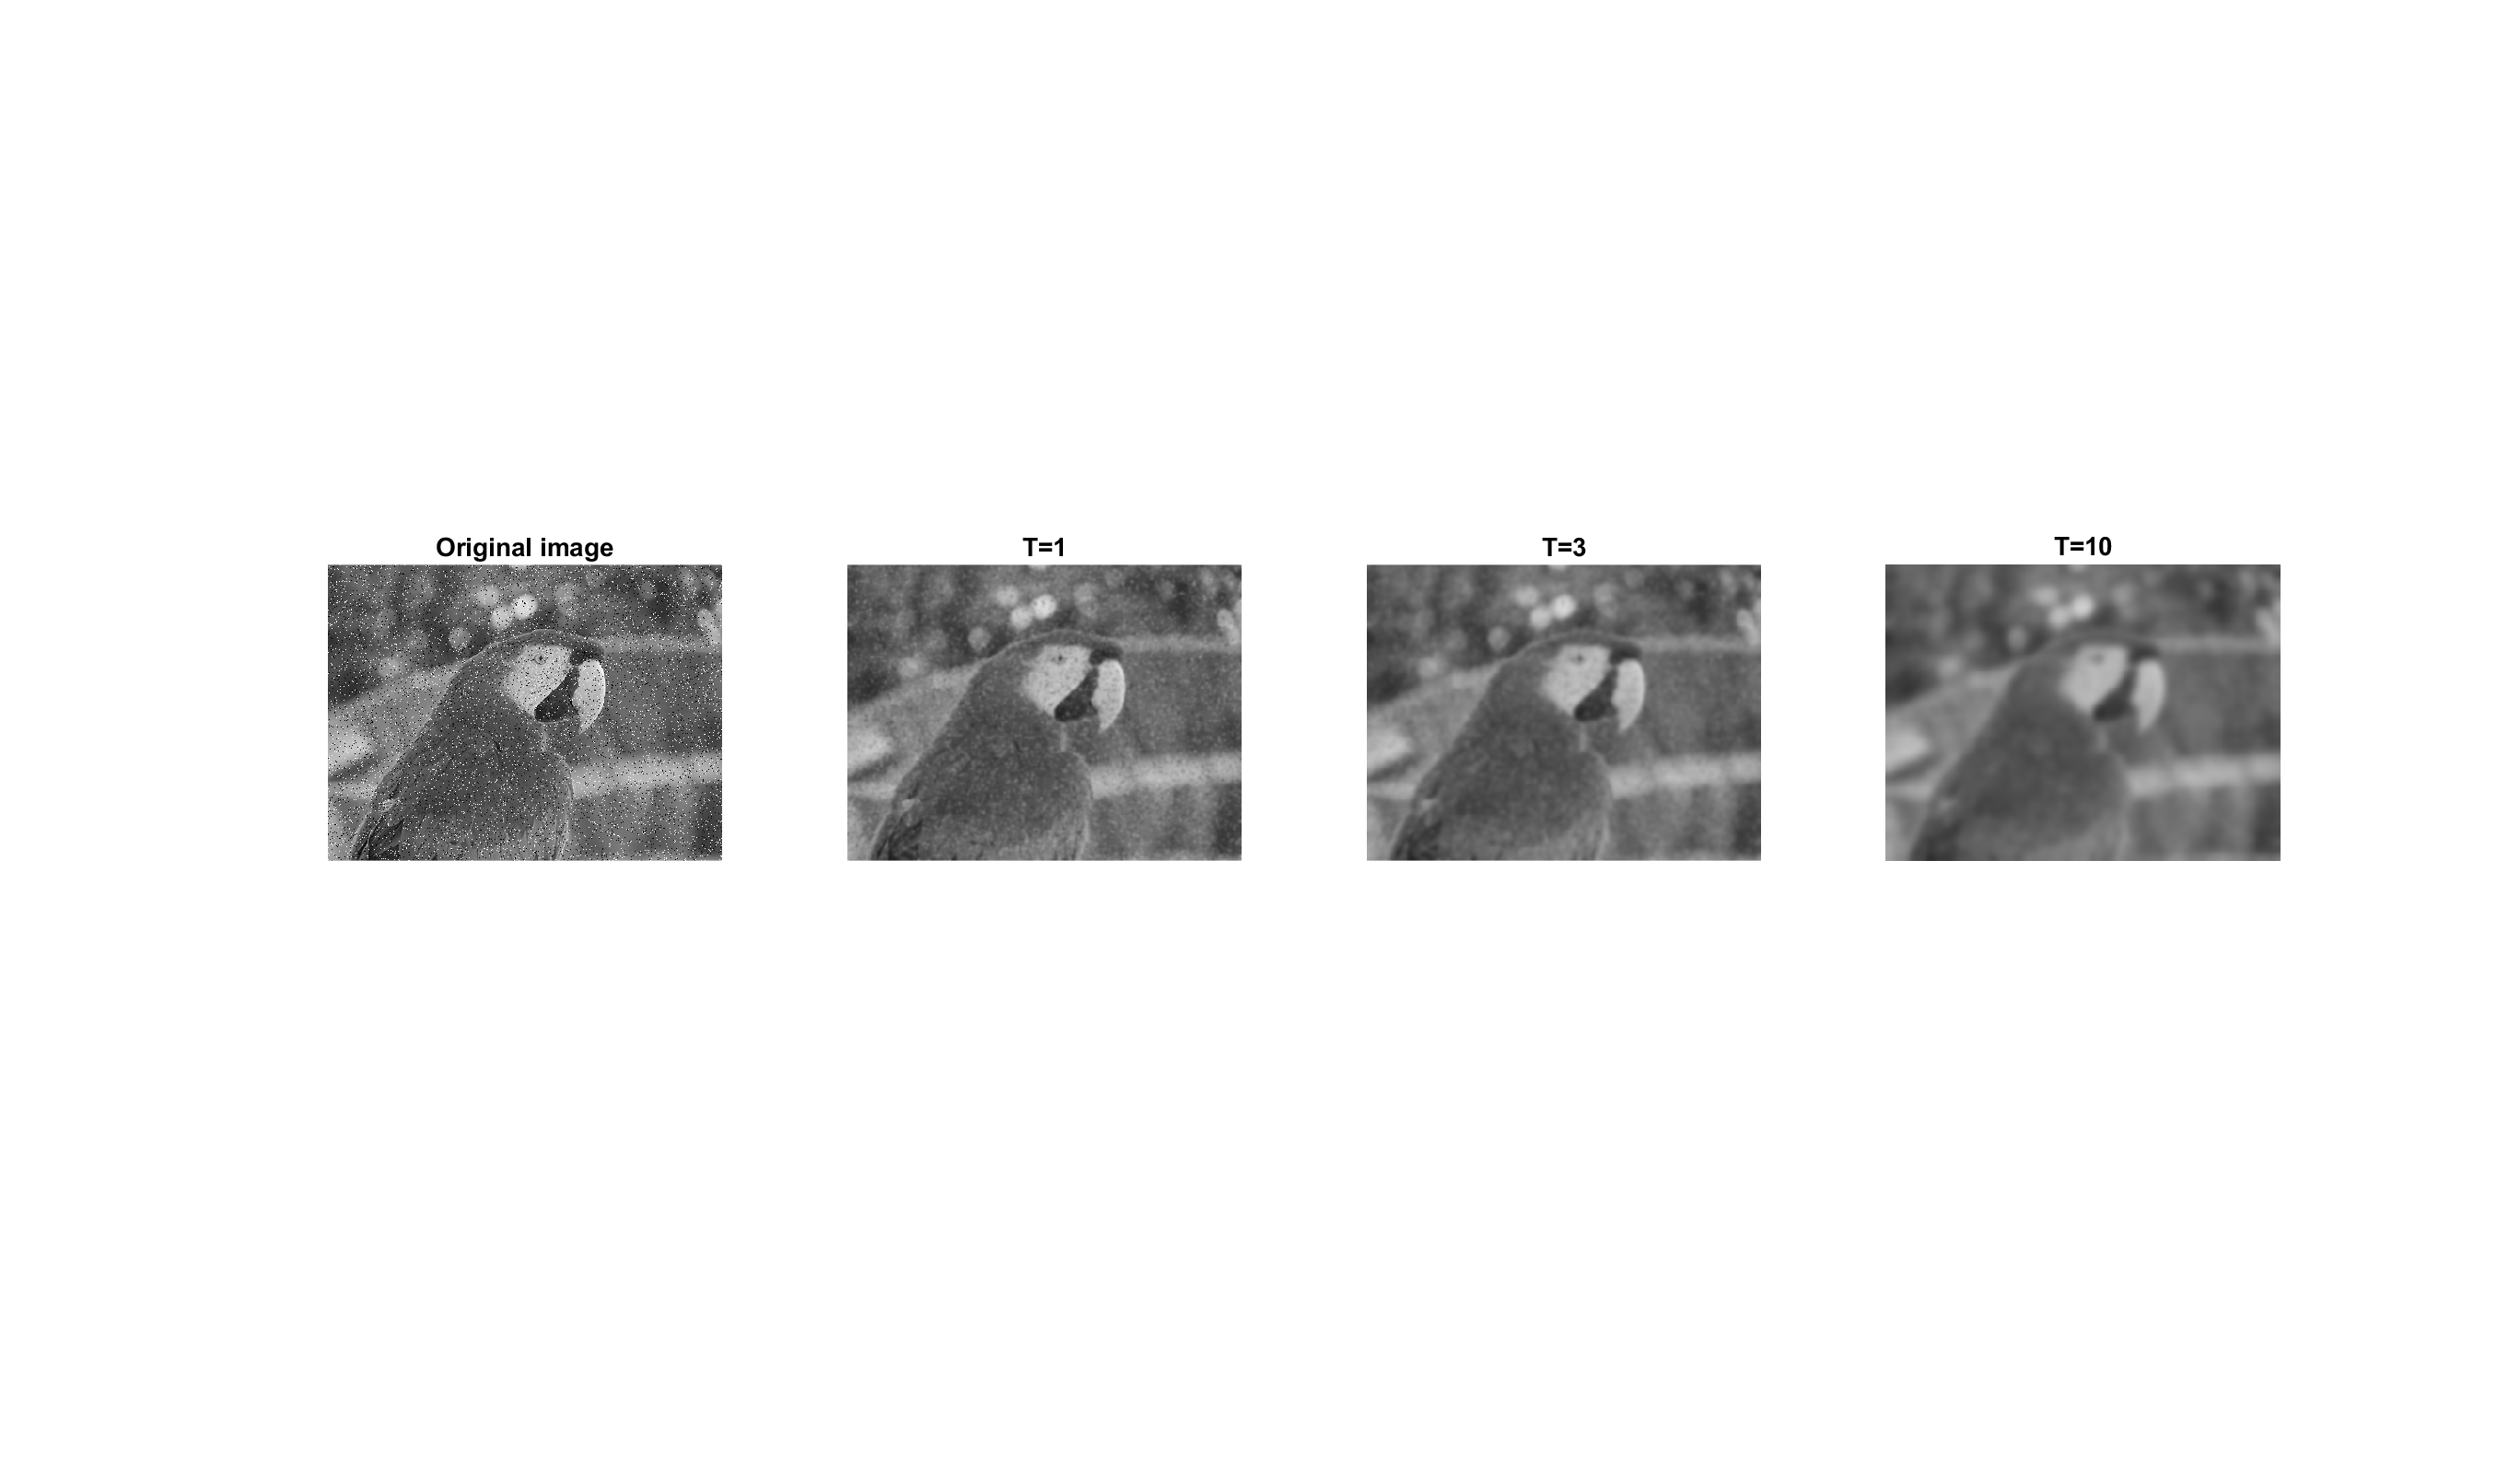
\includegraphics[scale=0.255, trim = 8.9cm 16.9cm 6.9cm 14.9cm, clip]{Pictures/Risultati/eq del calore_striscia.png}
%\includegraphics[scale=0.27, trim = 1.9cm 0.0cm 1.9cm 0.6cm, clip]{Pictures/Risultati/eq del calore 1.png}
%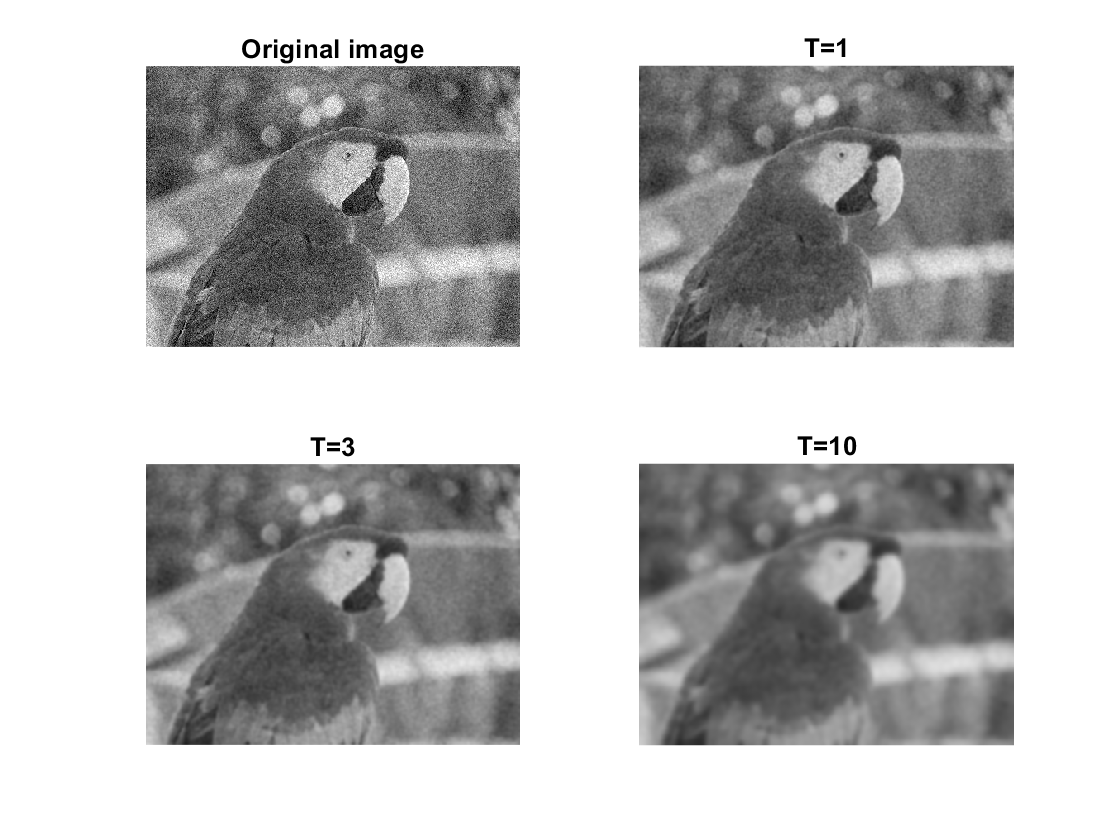
\includegraphics[scale=0.27, trim = 1.9cm 1.3cm 1.9cm 10.3cm, clip]{Pictures/Risultati/eq del calore.png}
\caption{Effetti dell'equazione del calore nel tempo.}\label{fig:figura}
\end{figure}


Questo metodo però ha un importante difetto, il rumore viene effettivamente eliminato o almeno ridotto ma si perdono importanti dettagli. In particolare, i margini degli oggetti presenti nell'immagine tendono progressivamente ad attenuarsi, come diretta conseguenza delle proprietà di regolarizzazione della soluzione dell'equazione del calore. Esistono tuttavia procedimenti come il metodo Perona-Malik che sono decisamente più efficaci.\\


\subsection{Studio della stabilità del metodo}
La tecnica delle differenze finite fornisce uno schema numerico che non è incondizionatamente stabile. Per studiare la sua stabilità e, conseguentemente, la sua convergenza, (grazie al teorema di equivalenza di Lax) utilizziamo un metodo classico per lo studio delle approssimazioni per le PDE:  il metodo di Von Neumann.\footnote{\cite{stab}}\\
Il metodo di Von Neuman si basa sulla decomposizione degli errori in serie di Fourier\\
Prima di procedere con il calcolo è utile fare un'osservazione preliminare.
\begin{osservazione}
Noto che il problema è risolubile tramite la formula iterativa
$$
u_{i,j}^{n+1}=u_{i,j}^{n}+r_{x}(u_{i+1,j}^{n}-2u_{i,j}^{n}+u_{i-1,j}^{n})+r_{y}(u_{i,j+1}^{n}-2u_{i,j}^{n}+u_{i,j-1}^{n})
$$
essa può essere riscritta come
$$
u_{i,j}^{n+1}=\frac{1}{2}u_{i,j}^{n}+r_{x}(u_{i+1,j}^{n}-2u_{i,j}^{n}+u_{i-1,j}^{n})+\frac{1}{2}u_{i,j}r_{y}(u_{i,j+1}^{n}-2u_{i,j}^{n}+u_{i,j-1}^{n})
$$
risultando essere somma di due fattori speculari riguardanti le due coordinate, possiamo quindi ragionevolmente effettuare i calcoli per una delle due parti e i risultati saranno coerenti anche nell'altra parte.\\
Detto $\epsilon=N-u$ l'errore dove u è la soluzione calcolata dall'algoritmo in precisione infinita e N è la soluzione calcolata in precisione finita di calcolo, allora
\hspace{0.5em}
$u_{j}^{n+1}=\frac{1}{2}u_{j}^{n}+r(u_{j+1}^{n}-2u_{j}^{n}+u_{j-1}^{n})$
e
$N_{j}^{n+1}=\frac{1}{2}N_{j}^{n}+r(N_{j+1}^{n}-2N_{j}^{n}+N_{j-1}^{n})$
da cui 
\hspace{-0.25em}
$$
\epsilon_{j}^{n+1}=N_{j}^{n+1}-u_{j}^{n+1}=\frac{1}{2}N_{j}-\frac{1}{2}u_{j}^{n}+r(N_{j+1}-u_{j+1}^{n}-2N_{j}+2u_{j}^{n}+N_{j-1}-u_{j-1}^{n})=\frac{1}{2}\epsilon _{j}^{n}+r(\epsilon_{j+1}^{n}-2\epsilon _{j}^{n}+\epsilon _{j-1}^{n})
$$
Sommando le due parti ritroviamo
$$
\epsilon_{i,j}^{n+1}=\epsilon_{i,j}^{n}+r_{x}(\epsilon_{i+1,j}^{n}-2\epsilon_{i,j}^{n}+\epsilon_{i-1,j}^{n})+r_{y}(\epsilon_{i,j+1}^{n}-2\epsilon_{i,j}^{n}+\epsilon_{i,j-1}^{n})
$$
questo dimostra che la soluzione e l'errore hanno lo stesso andamento.\\
\end{osservazione}
Questa osservazione, oltre a fornirci un risultato necessario per il calcolo che ci accingiamo a fare, ci introduce al ragionamento per \textit{separazione delle variabili} che utilizzeremo nella dimostrazione della proposizione seguente ed è molto utile per semplificare i calcoli.\\
\begin{proposizione}
il problema
$$
u_{i,j}^{n+1}=u_{i,j}^{n}+r_{x}(u_{i+1,j}^{n}-2u_{i,j}^{n}+u_{i-1,j}^{n})+r_{y}(u_{i,j+1}^{n}-2u_{i,j}^{n}+u_{i,j-1}^{n})
$$
dove $r_x=k_x\frac{\Delta t}{(\Delta x)^2}$ e $r_y=k_y\frac{\Delta t}{(\Delta y)^2}$, risulta stabile $\Leftrightarrow r_x+r_y\leq\frac{1}{2}$ 
\end{proposizione}
\begin{proof}

Senza ledere di generalità, consideriamo il caso dell'equazione del calore \textbf{uno-dimensionale}, come visto essa può essere discretizzata come:
$$
u_{j}^{n+1}=u_{j}^{n}+r(u_{j+1}^{n}-2u_{j}^{n}+u_{j-1}^{n})
$$
dove $r=k \frac{\Delta t}{(\Delta x)^2}$.\\


%Per le equazioni differenziali lineari con condizioni al contorno periodiche, la variazione spaziale dell'errore può essere espansa in una serie finita di Fourier rispetto a x nell'intervallo L, cioè
%$$
%\epsilon (x,t)=\sum _{m=-M}^{M}E_{m}(t)e^{{i}k_{m}x}
%$$
%dove $k_{m}={\frac {\pi m}{L}}$ è il numero d'onda e $M=\frac{L}{\Delta x}$

La variazione spaziale dell'errore può essere espansa con un integrale di Fourier rispetto ad x, cioè:
$$
\epsilon (x,t)=\int _{\tilde{\nu}=-{\frac {\pi }{\Delta x}}}^{\tilde{\nu}={\frac {\pi }{\Delta x}}}E_{\tilde{\nu}}(t)e^{{i}\tilde{\nu}x}d\tilde{\nu}
$$
Essendo l'equazione lineare, il termine generico va come l'integrale stesso, ossia: 
$\epsilon _{j}^{n}=E_{\tilde{\nu}}(t)e^{i\tilde{\nu}_{m}x}$ da cui:\\
\vspace{0.5em}
$\epsilon _{j}^{n+1}=E_{\tilde{\nu}}(t+\Delta t)e^{i\tilde{\nu}x}$\\ 
$\epsilon _{j+1}^{n}=E_{\tilde{\nu}}(t)e^{i\tilde{\nu}(x+\Delta x)}$\\ 
$\epsilon _{j-1}^{n}=E_{\tilde{\nu}}(t)e^{i\tilde{\nu}(x-\Delta x)}$\\
Sostituindo questi valori in $\epsilon_{j}^{n+1}=\epsilon _{j}^{n}+r(\epsilon _{j+1}^{n}-2\epsilon _{j}^{n}+\epsilon _{j-1}^{n})$ si ottiene:

$$
E_{\tilde{\nu}}(t+\Delta t)e^{i\tilde{\nu}x}=E_{\tilde{\nu}}(t)e^{i\tilde{\nu}x}+r(E_{\tilde{\nu}}(t)e^{i\tilde{\nu}(x+\Delta x)}-2E_{\tilde{\nu}}(t)e^{i\tilde{\nu}}x+E_{\tilde{\nu}}(t)e^{i\tilde{\nu}(x-\Delta x)})
$$
Affinché il metodo sia stabile occorre che l'errore non aumenti mai, ossia che\\
\vspace{0.25em}
$|E_{\tilde{\nu}}(t+\Delta t)|\leq |E_{\tilde{\nu}}(t)| \Rightarrow |\frac{E_{\tilde{\nu}}(t+\Delta t)}{E_{\tilde{\nu}}(t)}|\leq 1$. Esplicitiamo quindi per $\frac{E_{\tilde{\nu}}(t+\Delta t)}{E_{\tilde{\nu}}(t)}$ ed otteniamo:

$$
\frac {E_{\tilde{\nu}}(t+\Delta t)}{E_{\tilde{\nu}}(t)}=1+r(e^{i\tilde{\nu}\Delta x}+e^{-i\tilde{\nu}\Delta x}-2).
$$
detto $\theta =\tilde{\nu}\Delta x$, ricordo $\tilde{\nu}\in [-\frac{\pi}{\Delta x},\frac{\pi}{\Delta x}] \Rightarrow \theta \in [-\pi ,\pi ]$
per cui l'equazione diventa
$$
\frac {E_{\tilde{\nu}}(t+\Delta t)}{E_{m}(t)}=1+r(e^{i\theta x}+e^{-i\theta}-2).
$$

Prendiamo ora in considerazione l'identità 
$$
\sin \left({\frac {\theta }{2}}\right)={\frac {e^{i\theta /2}-e^{-i\theta /2}}{2i}} \Rightarrow
\sin ^{2}\left({\frac {\theta }{2}}\right)=-{\frac {e^{i\theta }+e^{-i\theta }-2}{4}}
$$
alla luce di questa osservazione, l'equazione diventa:
$$
\frac {E_{\tilde{\nu}}(t+\Delta t)}{E_{\tilde{\nu}}(t)}=1-4r\sin^2(\frac{\theta}{2}).
$$

Come detto, il metodo è stabile $\Leftrightarrow|\frac{E_{\tilde{\nu}}(t+\Delta t)}{E_{\tilde{\nu}}(t)}|\leq 1$ ma visto che $\frac {E_{\tilde{\nu}}(t+\Delta t)}{E_{\tilde{\nu}}(t)}=1-4r\sin^2(\frac{\theta}{2})\Rightarrow$ il metodo risulta stabile $\Leftrightarrow|1-4r\sin^2(\frac{\theta}{2})|\leq1$. Esplicitando:
$$
-1\leq 1-4r\sin^2(\frac{\theta}{2})\leq 1 \Rightarrow-2\leq -4r\sin^2(\frac{\theta}{2})\leq 0 \Rightarrow 0\leq 4r\sin^2(\frac{\theta}{2})\leq 2
$$
ma $\sin^2(\frac{\theta}{2})\ge0$ $\forall\theta\Rightarrow$il metodo risulta stabile $\Leftrightarrow r\sin^2(\frac{\theta}{2})\leq\frac{1}{2}$ siccome $\sin^2(\frac{\theta}{2})\leq1$ $\forall\theta\Rightarrow$ la condizione è sicuramente soddisfatta se $r\leq\frac{1}{2}$.
Avendo definito $r=k \frac{\Delta t}{(\Delta x)^2} \Rightarrow$ condizione sufficiente affinché il metodo sia stabile è $k \frac{\Delta t}{(\Delta x)^2}\leq\frac{1}{2}$\\
\vspace{1em}
Nel caso 2-dimensionale la soluzione discreta della PDE è:
$$
u_{i,j}^{n+1}=u_{i,j}^{n}+r_{x}(u_{i+1,j}^{n}-2u_{i,j}^{n}+u_{i-1,j}^{n})+r_{y}(u_{i,j+1}^{n}-2u_{i,j}^{n}+u_{i,j-1}^{n})
$$
dove $r_{x}=k_x \frac{\Delta t}{(\Delta x)^2}$ e $r_{y}=k_y \frac{\Delta t}{(\Delta y)^2}$\\ per cui la condizione diventa $r_{x}+r_{y}=k_x \frac{\Delta t}{(\Delta x)^2}+k_y \frac{\Delta t}{(\Delta y)^2}\leq\frac{1}{2}$.\\

\end{proof}
Nel caso in esame $\Delta x=\Delta y=1$ e $ k_x=k_y \Rightarrow r_{x}+r_{y}=k \Delta t+k \Delta t\leq\frac{1}{2} \Rightarrow k\Delta t\leq \frac{1}{4}$.\\
\vspace{0.5em}
La condizione appena calcolata è detta \textbf{condizione di Courant-Friedrichs-Lewy} (abbreviato \textbf{CFL}) per le equazioni alle derivate parziali di tipo parabolico
